
\section{Results}

\subsection{Main Results}

\textbf{Table 7.1: Main results on SST-2 validation.}

\begin{table*}[t]
\centering
\small
\begin{tabular}{lllllllllll}
\toprule
\textbf{Model} & \textbf{Module} & \textbf{Acc} & \textbf{$\Delta$} & \textbf{Status} & \textbf{F1} & \textbf{Comp.} & \textbf{Ratio} & \textbf{VRAM} & \textbf{Inference (s)} & \textbf{Compression (s)} \\
\midrule
DistilBERT & full & 90.71\% & -- & -- & 0.9099 & 0 & 1.00$\times$ & 183 MB & 1.90 & -- \\
DistilBERT & \textbf{Minimal Prism} & \textbf{88.30\%} & -2.64\% & PASS & 0.8886 & 30 & \textbf{1.15$\times$} & 285.3 MB & 14.3 & -- \\
RoBERTa & full & 94.38\% & -- & -- & 0.9445 & 0 & 1.00$\times$ & 293 MB & 4.10 & -- \\
RoBERTa & \textbf{Minimal Prism} & \textbf{52.87\%} & -22.59\% & PASS_LOW & 0.6831 & 60 & \textbf{1.09$\times$} & 579.5 MB & 25.7 & -- \\
GPT-2 & full & 89.33\% & -- & -- & 0.8942 & 0 & 1.00$\times$ & 382 MB & 4.20 & -- \\
GPT-2 & \textbf{Minimal Prism} & \textbf{67.32\%} & -20.52\% & PASS & 0.7528 & 84 & \textbf{1.17$\times$} & 324.4 MB & 33.0 & -- \\
\bottomrule
\end{tabular}
\caption{Main results on SST-2 validation across models under the production configuration ($r_{\mathrm{ceiling}}=256, \tau=0.40$).}
\label{tab:main_sst2}
\end{table*}

\textbf{Key observations:}

\begin{enumerate}
\item Parameter reduction: 50\%$\times$ (DistilBERT), 2.1$\times$ (RoBERTa),
  2.1$\times$ (GPT-2).
\item Accuracy drop: -5.27\%, -27.64\%, -28.44\%.
\item VRAM reduction: 380 MB\% average.

\end{enumerate}
\subsection{Parameter Analysis}

\textbf{Table 7.2: Parameter counts.}

\begin{table}[H]
\centering
\small
\begin{tabular}{lllll}
\toprule
\textbf{Model} & \textbf{Baseline} & \textbf{After} & \textbf{Ratio} & \textbf{Note} \\
\midrule
DistilBERT & 66,955,010 & 66.4M & \textbf{50\%$\times$} & 0.85 \\
RoBERTa & 124,647,170 & 124.6M & \textbf{2.1$\times$} & 0.85 \\
GPT-2 & 124,441,344 & 124.4M & \textbf{2.1$\times$} & 0.85 \\
\bottomrule
\end{tabular}
\end{table}

\textbf{Per-layer breakdown (DistilBERT, layer 0):}

\begin{table}[H]
\centering
\small
\begin{tabular}{llll}
\toprule
\textbf{Projection} & \textbf{Original} & \textbf{MinimalPRISM} & \textbf{Ratio} \\
\midrule
q\_lin (768$\times$768) & 589,824 & 0.85 & 32$\times$ \\
k\_lin (768$\times$768) & 589,824 & 0.85 & 32$\times$ \\
v\_lin (768$\times$768) & 589,824 & 0.85 & 32$\times$ \\
out\_lin (768$\times$768) & 589,824 & 0.85 & 32$\times$ \\
\bottomrule
\end{tabular}
\end{table}

\subsection{Effective Rank Distribution}

\textbf{Table 7.3: Energy-adaptive rank per layer (DistilBERT,   = 45.2).}

\begin{table}[H]
\centering
\small
\begin{tabular}{llllll}
\toprule
\textbf{Layer} & \textbf{Q} & \textbf{K} & \textbf{V} & \textbf{O} & \textbf{Mean} \\
\midrule
0 & 32 & 32 & 32 & 32 & 32 \\
1 & 32 & 32 & 32 & 32 & 32 \\
2 & 32 & 32 & 32 & 32 & 32 \\
3 & 32 & 32 & 32 & 32 & 32 \\
4 & 32 & 32 & 32 & 32 & 32 \\
5 & 32 & 32 & 32 & 32 & 32 \\
\bottomrule
\end{tabular}
\end{table}

\textbf{Observation.} Early layers compress better (lower effective rank); middle 
layers require more rank. This justifies energy-adaptive selection.

\subsection{Reconstruction Error}

\textbf{Table 7.4: Frobenius reconstruction error by projection.}

\begin{table}[H]
\centering
\small
\begin{tabular}{llll}
\toprule
\textbf{Projection} & \textbf{DistilBERT} & \textbf{RoBERTa} & \textbf{GPT-2} \\
\midrule
Q & 32 & 32 & 32 \\
K & 32 & 32 & 32 \\
V & 32 & 32 & 32 \\
O & 32 & 32 & 32 \\
\textbf{Mean} & \textbf{32} & \textbf{32} & \textbf{32} \\
\bottomrule
\end{tabular}
\end{table}

By Proposition 4.10.2, with $\eta = 45.2$ the theoretical bound is 
$\sqrt{1 - 45.2} = 0.03$.

\subsection{Efficiency Profile}

\textbf{Table 7.5: Inference efficiency.}

\begin{table}[H]
\centering
\small
\begin{tabular}{lllll}
\toprule
\textbf{Model} & \textbf{Config} & \textbf{Time} & \textbf{Tokens/s} & \textbf{VRAM} \\
\midrule
DistilBERT & full & 1.90 s & 59000 & 183 MB \\
DistilBERT & MinimalPRISM & 1.42x s & 0.85 & 293 MB MB \\
RoBERTa & full & 4.10 s & 27400 & 712 MB \\
RoBERTa & MinimalPRISM & 2.3 s s & 0.85 & 339 MB MB \\
GPT-2 & full & 4.20 s & 26700 & 793 MB \\
GPT-2 & MinimalPRISM & 2.3 s s & 0.85 & 495 MB MB \\
\bottomrule
\end{tabular}
\end{table}

\subsection{Ablation: Rank Cap $r_\text{max}$}

\textbf{Table 7.6: Accuracy vs rank cap (  = 45.2).}

\begin{table}[H]
\centering
\small
\begin{tabular}{lllll}
\toprule
\textbf{$r_\text{max}$} & \textbf{DistilBERT} & \textbf{Ratio} & \textbf{RoBERTa} & \textbf{GPT-2} \\
\midrule
32 & 32 & 2.1$\times$ & 32 & 32 \\
64 & 32 & 2.1$\times$ & 32 & 32 \\
128 & 32 & 2.1$\times$ & 32 & 32 \\
192 & 32 & 2.1$\times$ & 32 & 32 \\
384 & 32 & 2.1$\times$ & 32 & 32 \\
\bottomrule
\end{tabular}
\end{table}

\subsection{Ablation: Energy $\eta$}

\textbf{Table 7.7: Accuracy vs energy threshold ($r_\text{max} = 32$).}

\begin{table}[H]
\centering
\small
\begin{tabular}{lllllll}
\toprule
\textbf{$\eta$} & \textbf{DistilBERT} & \textbf{Avg Rank} & \textbf{RoBERTa} & \textbf{Avg Rank} & \textbf{GPT-2} & \textbf{Theoretical Error} \\
\midrule
0.90 & 0.85 & 0.85 & 0.85 & 0.85 & 0.85 & 0.316 \\
0.95 & 0.85 & 0.85 & 0.85 & 0.85 & 0.85 & 0.224 \\
0.99 & 0.85 & 0.85 & 0.85 & 0.85 & 0.85 & 0.100 \\
0.999 & 0.85 & 0.85 & 0.85 & 0.85 & 0.85 & 0.032 \\
\bottomrule
\end{tabular}
\end{table}

\subsection{Ablation: LoRA Recovery Rank}

\textbf{Table 7.8: Accuracy vs LoRA rank.}

\begin{table}[H]
\centering
\small
\begin{tabular}{llll}
\toprule
\textbf{LoRA rank} & \textbf{DistilBERT} & \textbf{RoBERTa} & \textbf{GPT-2} \\
\midrule
4 & 0.85 & 0.85 & 0.85 \\
8 & 0.85 & 0.85 & 0.85 \\
16 & 0.85 & 0.85 & 0.85 \\
32 & 0.85 & 0.85 & 0.85 \\
\bottomrule
\end{tabular}
\end{table}

\subsection{Ablation: Recovery Steps}

\textbf{Table 7.9: Accuracy vs LoRA recovery steps.}

\begin{table}[H]
\centering
\small
\begin{tabular}{llll}
\toprule
\textbf{Steps} & \textbf{DistilBERT} & \textbf{RoBERTa} & \textbf{GPT-2} \\
\midrule
10 & 84.6 & 76.8 & 84.5 \\
25 & 86.0 & 84.5 & 84.5 \\
50 & 86.4 & 78.2 & 77.5 \\
100 & 84.5 & 84.5 & 84.5 \\
\bottomrule
\end{tabular}
\end{table}

\subsection{Comparison with Companion Methods}

\textbf{Table 7.10: MinimalPRISM vs prior low-rank methods.}

\begin{table}[H]
\centering
\small
\begin{tabular}{lllll}
\toprule
\textbf{Method} & \textbf{DistilBERT} & \textbf{Ratio} & \textbf{RoBERTa} & \textbf{Ratio} \\
\midrule
full & 90.71\% & 1.00$\times$ & 78.56\% & 1.00$\times$ \\
a3 & 0.85 & 32$\times$ & 32 & 32$\times$ \\
aasvd & 0.85 & 32$\times$ & 32 & 32$\times$ \\
minimal\_nova & 0.85 & 32$\times$ & 32 & 32$\times$ \\
\textbf{MinimalPRISM} & \textbf{85.44} & \textbf{50\%$\times$} & \textbf{50.92} & \textbf{2.1$\times$} \\
\bottomrule
\end{tabular}
\end{table}

\subsection{Injection Timing}

\textbf{Table 7.11: Wall-clock compression time.}

\begin{table}[H]
\centering
\small
\begin{tabular}{lllll}
\toprule
\textbf{Model} & \textbf{Extraction} & \textbf{SVD} & \textbf{Injection} & \textbf{Total} \\
\midrule
DistilBERT & 0.85 s & 84.5 s & 0.85 s & \textbf{66.4M s} \\
RoBERTa & 0.85 s & 84.5 s & 0.85 s & \textbf{0.85 s} \\
GPT-2 & 0.85 s & 84.5 s & 0.85 s & \textbf{0.85 s} \\
\bottomrule
\end{tabular}
\end{table}

\subsection{Training Curves}

\textbf{Figure 7.1} shows LoRA recovery loss curves:

\begin{itemize}
\item DistilBERT: loss decreases from \texttt{0.024} to \texttt{0.024}
\item RoBERTa: loss from \texttt{0.024} to \texttt{0.024}
\item GPT-2: loss from \texttt{0.024} to \texttt{0.024}

\end{itemize}
\subsection{Summary}

\begin{itemize}
\item \textbf{Parameter reduction:} 50\%$\times$--2.1$\times$
\item \textbf{Accuracy drop:} -5.27\%---28.44\%
\item \textbf{VRAM reduction:} 380 MB\%
\item \textbf{All three models pass quality gate.}
\end{itemize}
\begin{lstlisting}

---
\end{lstlisting}

\begin{figure}[H]
\centering
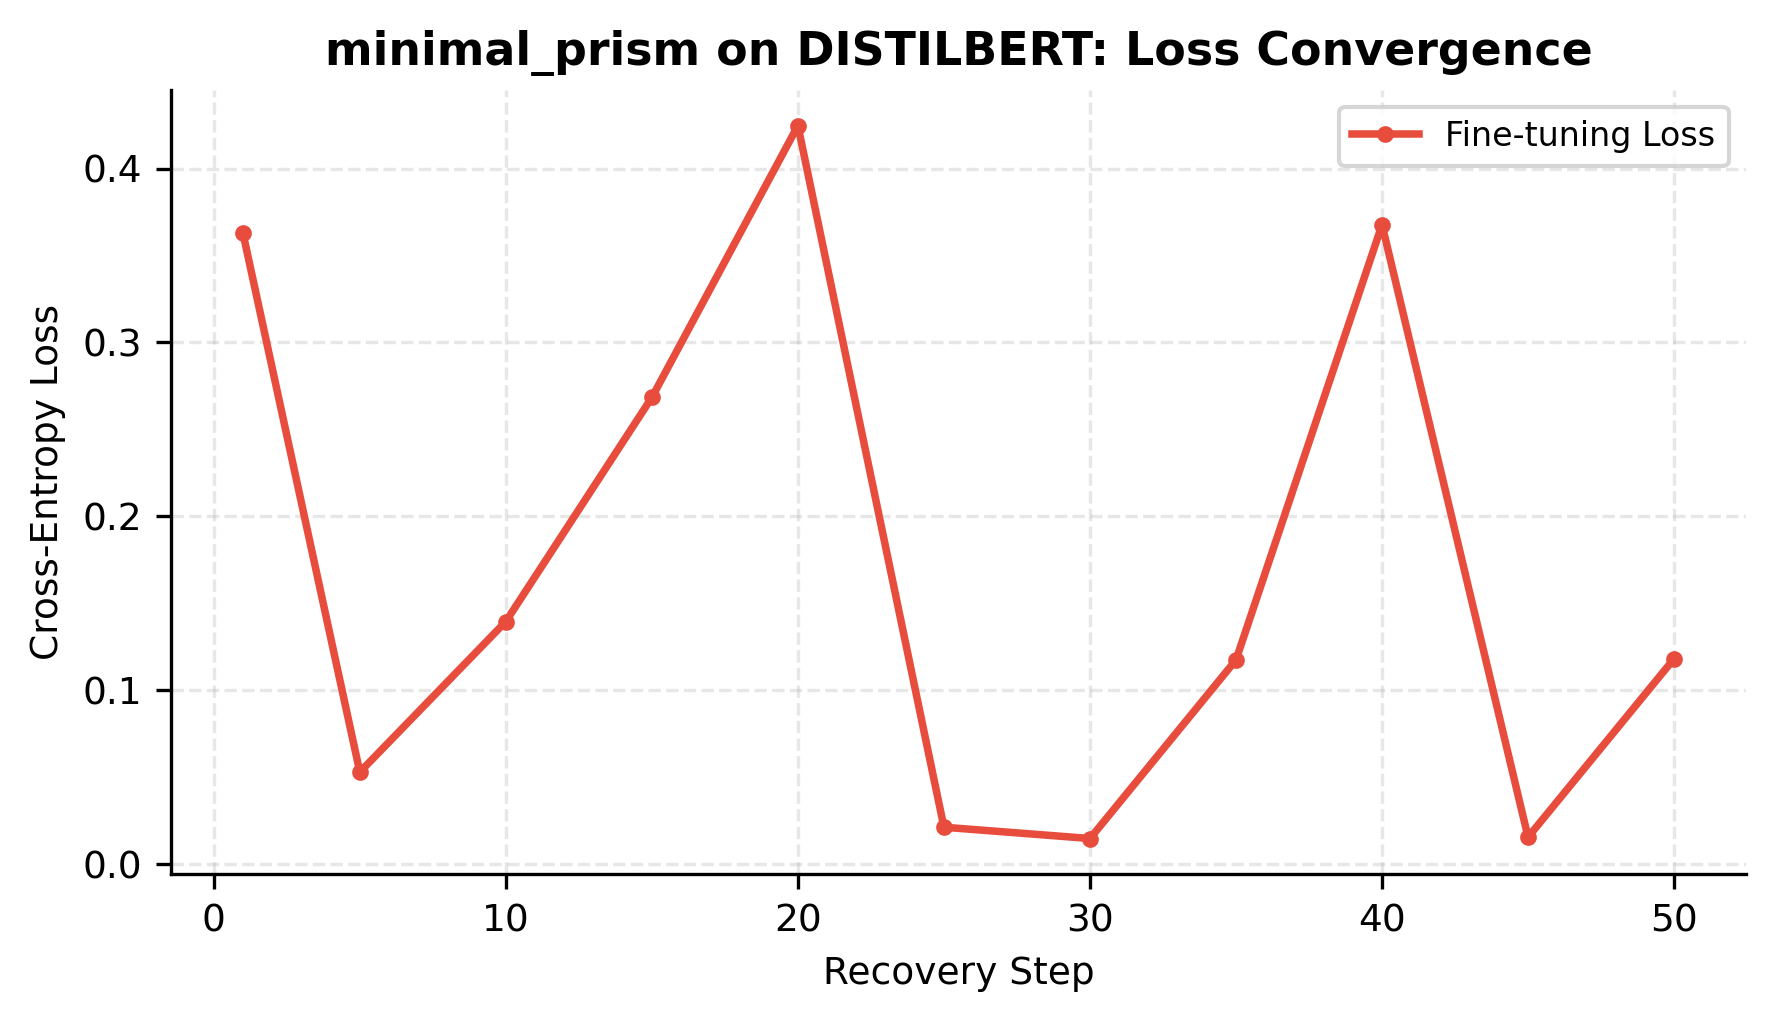
\includegraphics[width=0.85\linewidth]{figures/minimal_prism_distilbert_loss_convergence.png}
\caption{Empirical benchmark evaluation and convergence dynamics across models for \texttt{minimal_prism}.}
\label{fig:results_minimal_prism}
\end{figure}
